\documentclass[12pt,a4paper]{article}
\usepackage[utf8]{inputenc}
\usepackage[english]{babel}
\usepackage{enumerate}
\usepackage{amsmath}
\usepackage{amsfonts}
\usepackage{amssymb}
\usepackage{graphicx}
\usepackage{fourier}
\usepackage[left=2cm,right=2cm,top=2cm,bottom=2cm]{geometry}
\usepackage{commath}
\usepackage{cancel}
\usepackage{placeins}
\author{Juan Carlos Apitz, ID 012523821}
\title{STAT572 - Homework Assignment 4}
\begin{document}

\maketitle

\section*{In-class 4: Monte Carlo Hypothesis Testing for $\hat{\sigma}$}
\textbf{MATLAB Code:}
\begin{verbatim}
% In-class; hypothesis test on the standard deviation parameter

load mcdata; n = length(mcdata);  								
% Population sigma is known.
sigma = 7.8; sigxbar = sigma/sqrt(n);
% Get the observed value of the test statistic.
Tobs = (n-1)*var(mcdata)/sigma^2;

M = 1000; % Number of Monte Carlo trials
Tm = zeros(1,M);
% Start the simulation.
for i = 1:M
			% Generate a rand sample under H_0 where n is the sample size.
			xs = sigma*randn(1,n) + mean(mcdata);
			Tm(i) = (n-1)*var(xs)/sigma^2;
end

% This is a upper-tail test, so it is the 1-alpha quantile.
alpha = 0.05; cv = csquantiles(Tm,1-alpha);

% Plotting in-class
figure(2); hist(Tm)
set(get(gca,'child'),'FaceColor',[.9 .9 .9],'EdgeColor','black');
hold on
plot(cv,0,'*',Tobs,0,'bo')
legend('frequency','critical value','observed value')
hold off

% Calculating the p-value
g = [];
for i=1:length(Tm)
    if Tm(i) >= Tobs
        g = [g,Tm(i)];
    end
end
pval=length(g)/length(Tm);
\end{verbatim}

The p-value calculated by the above algorithm is $0.2600$. Given that we chose $\alpha=0.05$, we fail to reject $H_o:$ $\sigma=7.8$ in favor of the alternative $H_a:$ $\sigma>7.8$.

\begin{figure}[ht!] 
\begin{center}
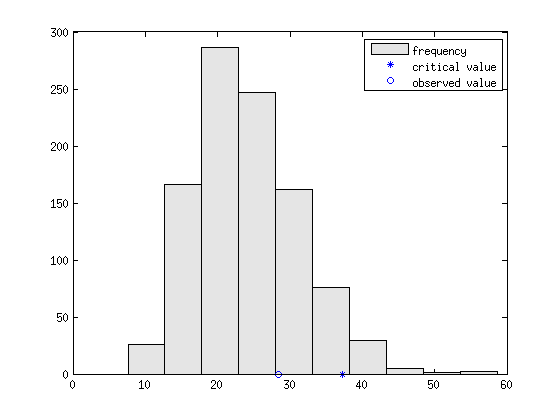
\includegraphics[scale=1]{inClass4_hist.png}
\caption{}
\label{inclass4 fig1}
\end{center}
\end{figure}
\FloatBarrier

\section*{In-class 5: Bootstrap Exercise on the Mean and 10\% Trimmed Mean}

\textbf{MATLAB Code:}

\begin{verbatim}
% generate 200 rs from chi-square df=f
X = chi2rnd(5,1,200);

% PART A
n = length(X); % sample size
B = 400;	% number of bootstrap replicates
% Get the value of the statistic of interest.
theta = mean(X);

% Use unidrnd to get the indices to the resamples.
inds = unidrnd(n,n,B);
% Extract these from the data.
xboot = X(inds);
thetab = mean(xboot); % get the mean for each column using
seb = std(thetab);
biasEst = mean(thetab)-theta;

figure(1)
hist(thetab)
set(get(gca,'child'),'FaceColor',[.9 .9 .9],'EdgeColor','black');
title('Boostrapped Sample Mean Histogram')
ylabel('Frequency');  xlabel('Sample mean')

% PART B
thetat = trimmean(X,10); % use MATLAB trimmed mean function to estimate 
thetatb = trimmean(xboot,10); % generate boostrap trimmed mean
sebt = std(thetatb); % calculate the boostrap standard error
biastEst = mean(thetatb)-thetat; % estimate the bias

figure(2)
hist(thetatb)
set(get(gca,'child'),'FaceColor',[.9 .9 .9],'EdgeColor','black');
title('Boostrapped Trimmed Mean Histogram')
ylabel('Frequency'); xlabel('Trimmed mean')

par={'Sample Mean';'Trimmed Mean'}; Value = [mean(thetab); mean(thetatb)];
StdError = [seb; sebt]; Bias = [biasEst; biastEst];
T=table(Value,StdError,Bias,'RowNames',par); disp(T)

\end{verbatim}

Implementing the above code we estimate the parameter, standard error and bias. This information is presented in figure \ref{inclass5 fig1}. The histograms are presented in figures \ref{inclass5 fig2} and \ref{inclass5 fig3}.

\begin{figure}[ht!]
\begin{center}
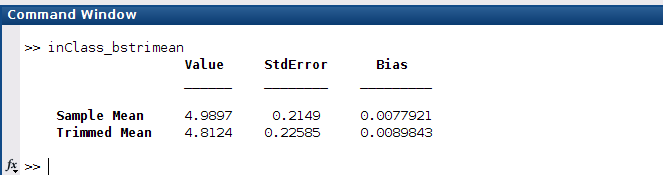
\includegraphics[scale=.6]{inClass5_code2.png}
\caption{Mean and Trimmed Mean results.}
\label{inclass5 fig1}
\end{center}
\end{figure}
\FloatBarrier

\begin{figure}[ht!]
\begin{center}
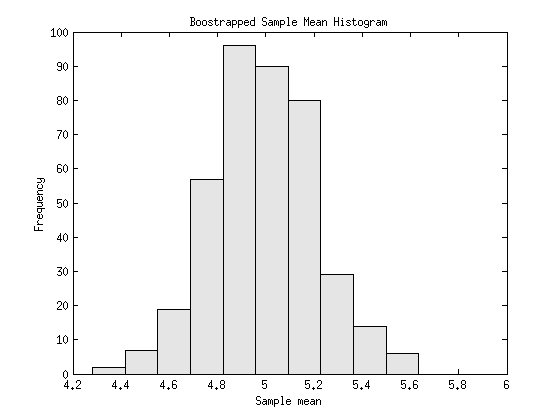
\includegraphics[scale=.8]{inClass5_mhist.png}
\caption{Frequency Histogram of the Bootstrapped Mean Parameter}
\label{inclass5 fig2}
\end{center}
\end{figure}
\FloatBarrier

\begin{figure}[ht!]
\begin{center}
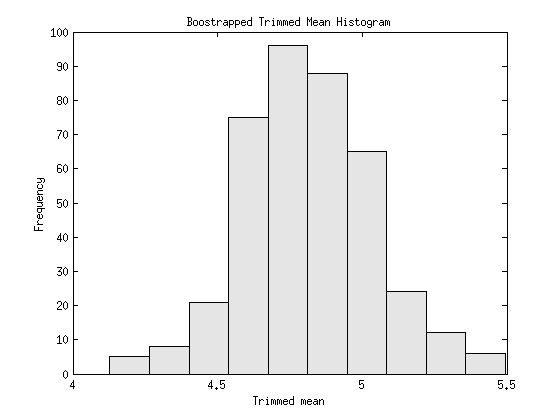
\includegraphics[scale=.8]{inClass5_thist.png}
\caption{Frequency Histogram of the Bootstrapped 10\% Trimmed Mean Parameter}
\label{inclass5 fig3}
\end{center}
\end{figure}
\FloatBarrier

\section*{Exercise 7.2}

\textbf{MATLAB Code:}

\begin{verbatim}
% Based on Example 7.3 - Matinez

% Get several values for the mean under the alternative
% hypothesis. Note that we are getting some values
% below the null hypothesis.
mualt = 40:60;

% Note the critical value:
cv = 1.645;
% Note the standard deviation for x-bar:
sig = 1.5;
% It's easier to use the unstandardized version, 
% so convert:
ct = cv*1.5 + 45;

% Get a vector of ct values that is 
% the same size as mualt.
ctv = ct*ones(size(mualt));
% Now get the probabilities to the left of this value.
% These are the probabilities of the Type II error.
beta = normcdf(ctv,mualt,sig);

% Plot probablity of a type II error vs. true mean
% under the alternative hypothesis
plot(mualt,beta);
xlabel('True Mean \mu')
ylabel('Probability of Type II Error')
axis([40 60 0 1.1])

\end{verbatim}

In figure \ref{q7p2 fig1} below we see the relationship between the probability of a Type II Error and different values of the mean under the alternative hypothesis. We see precisely the opposite relationship between the power of the test, i.e. $1-\beta$, and the means under the alternative which is shown in example 7.3 in the book (Martinez). This expected because of the definition Power$=1-\beta$ and probability of a Type II Error$=\beta$.

\begin{figure}[ht!]
\begin{center}
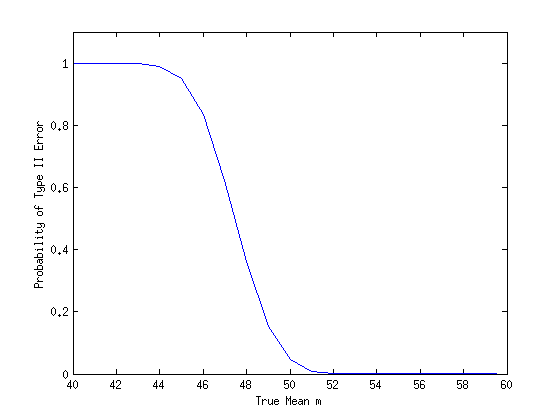
\includegraphics[scale=.75]{q7p2_graph.png}
\caption{As the true mean of the population under the alternative hypothesis gets larger the probability of making a type II error goes to zero. This is precisely the opposite of the figure presented in example 7.3 in the book (Martinez).}
\label{q7p2 fig1}
\end{center}
\end{figure}
\FloatBarrier

\section*{Exercise 7.4}

\textbf{MATLAB Code:}

\begin{verbatim}
% Based on example 7.3

% Generate the mean under the alternative
mualt = 40:60;

% Note the critical value:
cv = 1.645;
% Note the standard deviation for x-bar:
sig=15./sqrt([50,100,200]);

% It's easier to use the unstandardized version, 
ct = cv.*sig + 45;

% Get a vector of ct values that is 
% the same size as mualt.
one = ones(size(mualt));
ctv = [ct(1)*one;ct(2)*one;ct(3)*one];

% Now get the probabilities to the left of this value.
% These are the probabilities of the Type II error.
beta50 = normcdf(ctv(1,:),mualt,sig(1));
beta100 = normcdf(ctv(2,:),mualt,sig(2));
beta200 = normcdf(ctv(3,:),mualt,sig(3));

% To get the power: 1-beta
pow50 = 1 - beta50;
pow100 = 1 - beta100;
pow200 = 1 - beta200;

plot(mualt,pow50,'r-o');
hold on
plot(mualt,pow100,'-*');
hold on
plot(mualt,pow200,'--');
xlabel('True Mean \mu')
ylabel('Power')
axis([40 60 0 1.1])
legend('Power for n=50','Power for n=100','Power for n=200',2)
hold off

\end{verbatim}

In figure \ref{q7p4 fig1} we see three different power curves for three different sample sizes, $n=50$, $n=100$ and $n=200$. Notice that the larger the sample size the greater the power of the test. For example, for every possible value of $\mu$ under the alternative, the curve corresponding to $n=200$ is above the other curves. Similarly, the curve that corresponds to $n=100$ is above the curve corresponding to $n=50$. This is expected given that the standard error of the sample mean is $\frac{\sigma}{\sqrt{n}}$. This tells us that the larger the sample size $n$, the smaller the standard error of the parameter estimate.

\begin{figure}[ht!]
\begin{center}
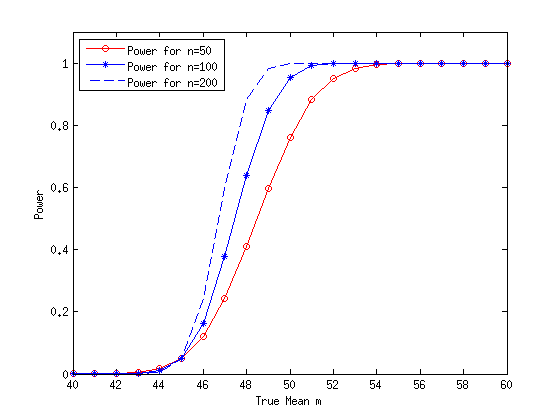
\includegraphics[scale=.75]{q7p4_graph.png}
\caption{Power of the test for $n=50,100,200$}
\label{q7p4 fig1}
\end{center}
\end{figure}
\FloatBarrier

\section*{Exercise 7.5}

\textbf{MATLAB Code}

\begin{verbatim}
% Two-tailed test for Example 7.6 

load mcdata
n = length(mcdata);  								
% Population sigma is known.
sigma = 7.8;					
sigxbar = sigma/sqrt(n);
% Get the observed value of the test statistic.
Tobs = (mean(mcdata)-454)/sigxbar;

% This command generates the normal probability plot.
normplot(mcdata)

M = 1000; % Number of Monte Carlo trials
	% Storage for test statistics from the MC trials.
	Tm = zeros(1,M);
	% Start the simulation.
for i = 1:M
			% Generate a random sample under H_0
			% where n is the sample size.
			xs = sigma*randn(1,n) + 454;
			Tm(i) = (mean(xs) - 454)/sigxbar;
end

% Get the critical value for alpha.
% This is a two-tail test, so we need the
% alpha and 1-alpha quantile.
alpha = 0.05/2;
cv1 = csquantiles(Tm,alpha);
cv2 = csquantiles(Tm,1-alpha);
fprintf('Critical Values\t\t%9.3f\t%9.3f\n',cv1,cv2)


\end{verbatim}

Implementing the above code allows us two get two critical values at the points where $P(X<x_l)=\alpha/2$ and $P(X>x_u)=\alpha/2$. The calculated values are $x_l=-1.891$ (lower) and $x_u=1.867$. The value $\alpha=0.05$. The resulting test statistic Tobs$=-2.5641$ thus we reject the null hypothesis in favor of the alternative that the mean is not equal to 454.  See figure \ref{q7p5 fig1} below for MATLAB output.

\begin{figure}[ht!]
\begin{center}
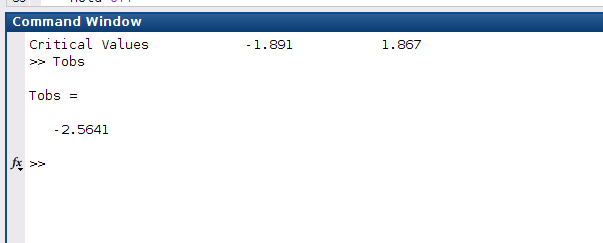
\includegraphics[scale=.75]{q7p5_result.png}
\caption{Empirical Critical Values}
\label{q7p5 fig1}
\end{center}
\end{figure}
\FloatBarrier

\section*{Exercise 7.6}

\textbf{MATLAB Code}

Exactly the same as Example 7.8 from the book. I only changed the variable M. I show just the initial part of the code:

\begin{verbatim}
% Example 7.8
clc
load mcdata; n = length(mcdata);  								
% Population sigma is known.
sigma = 7.8; sigxbar = sigma/sqrt(n);

M = 100000; alpha = 0.05;
% Get the critical value, using z as test statistic.
cv = norminv(alpha,0,1);
% Start the simulation.
\end{verbatim}
\vdots

Changing M increases the size of the sample generated by the simulation. This caused the estimation of the type I error, $\hat{\alpha}$ to approach its true value. Figure \ref{q7p6 fig1} shows the results for $M=1000$ and $M=100000$. As you can see the estimate when $M=100000$ is much closer to its true value, $\alpha=0.05$. The respective absolute differences from $\alpha=0.05$ are $0.4\times10^{-2}$, and $-0.3\times10^{-3}$.

\begin{figure}[ht!]
\begin{center}
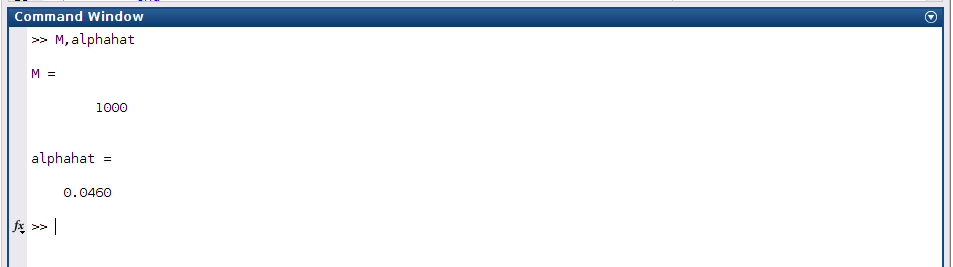
\includegraphics[scale=.5]{q7p6_result1.png}
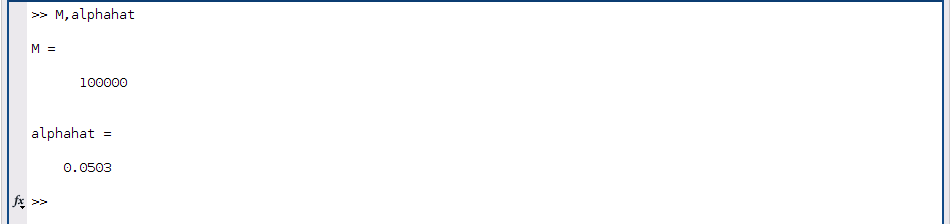
\includegraphics[scale=.5]{q7p6_result2.png}
\caption{}
\label{q7p6 fig1}
\end{center}
\end{figure}
\FloatBarrier

\section*{Exercise 7.7}

\textbf{MATLAB Code}

\begin{verbatim}
% Code for exercise 7.7

% get the dataset
load forearm;
% PART A
n = length(forearm); % sample size
B = 1000;	% number of bootstrap replicates
% Get the value of the statistic of interest.
theta1 = skewness(forearm);
theta2 = kurtosis(forearm);
theta3 = var(forearm,1);

% Use unidrnd to get the indices to the resamples.
inds = unidrnd(n,n,B);
% Extract these from the data.
foreboot = forearm(inds);
theta1b = skewness(foreboot); % get the skewnwness for each column using
theta2b = kurtosis(foreboot); % get the kurtosis for each column using
theta3b = var(foreboot,1); % get the 2nd moment for each column using

seb1 = std(theta1b);
seb2 = std(theta2b);
biasEst1 = mean(theta1b)-theta1;
biasEst2 = mean(theta2b)-theta2;

% PART B
% find the bootstrap percentile interval for the central 2nd moment
alpha = 0.1;
k = B*alpha/2;
theta3b = sort(theta3b);
blo = theta3b(k);
bhi = theta3b(B-k);

fprintf('Skewness Standard Error and Bias %9.3f\t%4.3f\n\n',seb1,biasEst1)
fprintf('Kurtosis Standard Error and Bias %9.3f\t%4.3f\n\n',seb2,biasEst2)
fprintf('Pct Interval for 2nd Central Moment (%2.3f, %3.3f)\n',blo,bhi)
\end{verbatim}

The resulting percentile interval is $1.029, 1.460)$ which means, based on the bootstrap procedure, given that $\alpha=0.1$, we should expect, on repeated sampling, that $90\%$ of the calculated sample 2nd central moments statistics will fall within this interval.

\begin{figure}[ht!]
\begin{center}
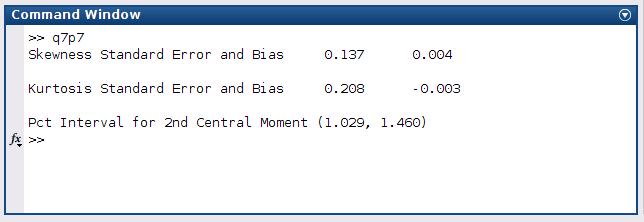
\includegraphics[scale=.6]{q7p7_result.png}
\caption{Results, exercise 7.7.}
\label{q7p7 fig1}
\end{center}
\end{figure}
\FloatBarrier

\section*{Exercise 7.11}

\textbf{MATLAB Code}

\begin{verbatim}
% Exercise 7.11
clear;
% load population data
load lawpop

% find true variances for the lsat and gpa populations
popVar = var(lawpop,1);

% load sample data
load law

% BOOTSTRAP Procedure
B = 10000;	% number of bootstrap replicates

% get the bootstrap values for the variance based on the sample data
bvals = bootstrp(B, @(x) var(x,1),law);

% get bootstrap estimates for the standar error and the bias
seb = std(bvals); biasb = mean(bvals)-popVar;

\end{verbatim}

The above code implements the bootstrap procedure and calculates bootstrap estimates of the variance, variance standard error, and bias. The MATLAB results are shown in figure \ref{q7p11 fig1} below. To get a sense of how well the bootstrap estimates perform, we look at the ratio of the standard error and the ratio of the bias as a percent of the corresponding population variance.  We can see that for the LSAT measure, the standard error is about $24\%$ of the true variance, while for the GPA measure the standard error is about $35\%$, hence the estimates of GPA variance are more dispersed around the true value. We note a similar result for the bias. The LSAT estimate bias is about $4\%$ of the true variance, while the estimate bias of GPA variance is about $46\%$ of the true parameter. We can see that the bootstrap variance estimate of LSAT is more stable that that of the GPA data.

\begin{figure}[ht!]
\begin{center}
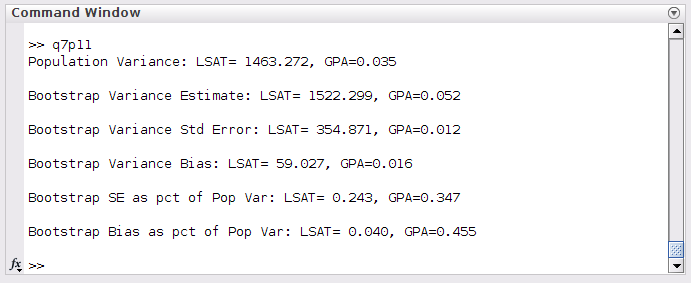
\includegraphics[scale=.6]{q7p11_result.png}
\caption{Results, exercise 7.11.}
\label{q7p11 fig1}
\end{center}
\end{figure}
\FloatBarrier

\end{document}